\section{Energy Profile Model}
In this section, we derive a model to characterize how the energy profile of each of the four states has evolved from 1960 – 2009, called the energy profile model. Specially, we state total energy consumption as the sum of fossil fuels energy, renewable energy and nuclear energy.
\subsection{Integrat variables}
First, we address the data according to the integrity and redundancy of the information. We divide energy into 4 major categories and 11 minor categories like what displayed in \autoref{tab:bianliang}. 
Then, we analyze the 50 years of data in 11 variables on each of these four states’ energy production and consumption. 
Since all forms of energy tend to eventually be converted into electricity, we temporarily ignore the effects of electricity imports and exports. To simplify the problem, we ignore trade between each state in the United States too. Fuel ethanol, wood and waste are partially coincidental with biomass.So we choose biomass as a representative. \\
\begin{table}[h]
	\begin{tabular}{ccc}%c的个数代表列数,这是典型的三线表样式。
		\toprule
		minor categories  & MSN & major categories(MSN) \\
		\midrule
		Oil and Petroleum Products & PMTCB& \\
		Coal & CLTCB & Fossil Fuels(FFTCB)\\
		Natural Gas & NNTCB & \\
		\midrule	
		Nuclear Energy &NUTCB& Nuclear Energy(NUTCB) \\
		\midrule
		Hydroelectricity & HYTCB &  \\
		Biomass &EMLCB+EMTCB &  \\
		Wind Energy& WYTCB & Renewable Energy(RETCB) \\
		Geothermal Energy 	&GETCB  &  \\
		Solar Energy 	& SOTCB&  \\
		\midrule
		Electricity &ESTCB&Electricity(ESTCB)\\
		\bottomrule                  
	\end{tabular}
	\caption{Energy Categories}                      %名称
	\label{tab:bianliang} 
\end{table}
%https://www.eia.gov/state/seds/sep_use/notes/use_a.pdf
Note: $ PMTCB  $ represents all petroleum products total consumption excluding fuel ethanol.\\
Note: we only use data from the provided excel table and that mentioned in the pdf file.
\begin{align}
FFTCB &= CLTCB + NNTCB + PMTCB\\
PMTCB &= PATCB - EMTCB
\end{align}
However, after screening the data, we found that, judging from the order of magnitude difference, fuel ethanol(excluding denaturant) accounts for a very small percentage of fossil fuels.The maximum was produced in California in 2009, but not more than 1.5\%.(AZ:1.48\%,CA: 1.37\%,NM: 0.51\%,TX: 0.64\%)At the same time, we found loss of the cost of all petroleum products total consumption excluding fuel ethanol.
Therefore, we use $ PATCB $ rather than $ PMTCB $ in \autoref{eq:shiyoudaiti}.
\begin{align}
FFTCB \approx CLTCB + NNTCB + PATCB\label{eq:shiyoudaiti}
\end{align}
%即ESTCP=REPRB-EMTCB+ELNIB+ELISB
%
%文中用到的变量在术语表中列出
%
%得到
%
%由RETCB=REPRB得到
%由于各行业的可再生能源消耗量(RETCB)、燃料乙醇,不含变性剂,总消耗量(EMTCB)、净电力进入美国量(ELNIB)、净州际电力销售和相关损失(ELISB)未知
%
%我们假设各上述部分能源按电能的消耗量比例分配
%这里给一个公式
%然后算下各行业的四大能源消耗量(电能净进口及贸易损失变成了电能)
%即我们在分析因素的时候分析的是化石燃料、可再生能源、核能以及电能的消耗量(根据行业、人口、地理等)
%
%
%表一只使用了,B-J 最后一列没有在制作面积图的时候考虑
%我等会儿会发行业能源消耗表用来①B题的分析因素,这部分@离宫 你找个插值补数的文章插进去,因为这个表的数据有极少缺失,我们认为是统计失误,用一下插值法,到时候再附段代码
%
%
%其实就是我们瞎编一个数值插进去就好了,毕竟只是分析一下(但表面工作要做的)
%
%而且缺失数据的那个项目对总体量影响非常小
%
%在四个州中,我们对风能,地热能,太阳能所占可再生资源所占的比例进行了分析,其中风能的所占比的最大值分别为:0.08%(2009),3.28%(2009),13.13%(2008),12.16%(2009)地热能最大值分别为:0.10%(1991),9.82%(1991),0.99%(2001年),0.13%(2009)太阳能:1.54%(1993)1.81%(2009)0.98%(1990)0.05%(2009)综合以上数据,以及新型能源的应用,我们考虑
%
%
%那个木材和废物加乙醇的那两个小的就是生物质能
%
%易水寒(573721927)  0:19:04
%我想把各行业对能源消耗影响程度(权重因子)作为一个指标@离宫 这个影响因子你可以加上这一句:该影响因子在一定程度上考虑了各州某个行业的能源利用率,即包含损耗在内

We analyze the data and use energy consumption as an indicator of energy profile in four states.\\
Then the energy configuration analysis we established is shown in \autoref{fig:mianjitu} as an area chart. (code seen in Appendix 1)\\
\begin{figure}[h]
	\centering                                             %居中
	\subfigure[Energy Structure of AZ]{                    %第一张子图
		\begin{minipage}{7cm}
			\centering                         %子图居中
			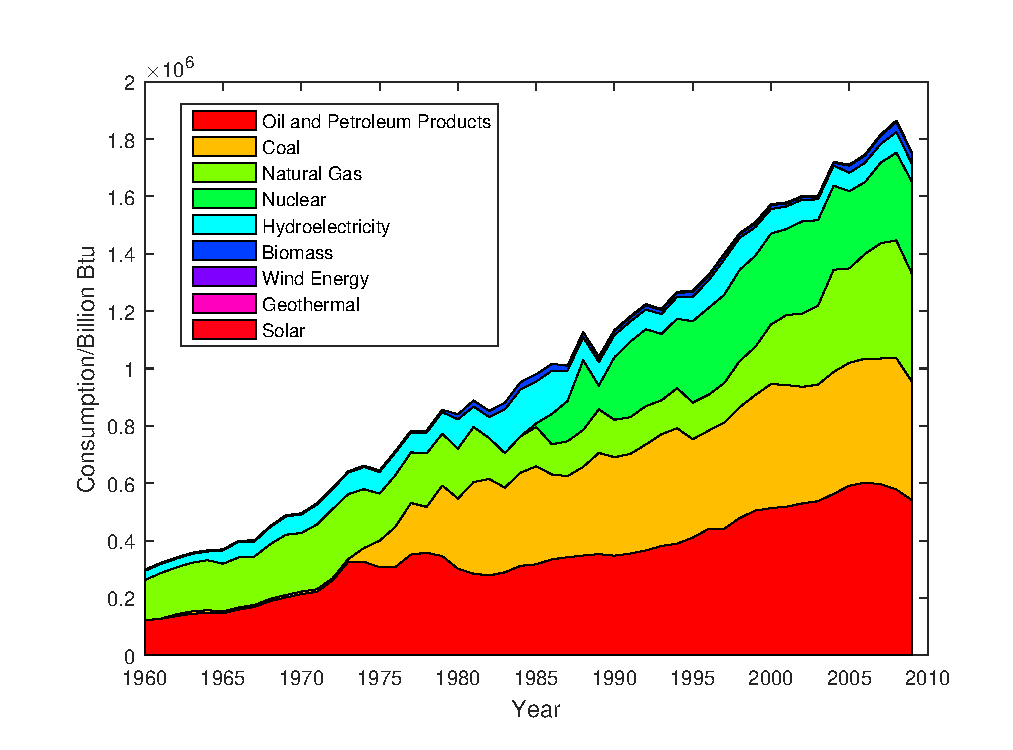
\includegraphics[scale=0.4]{figure/AZconsumption}    %以pic.jpg的0.5倍大小输出
		\end{minipage}}
	\subfigure[Energy Structure of CA ]{                    %第二张子图
		\begin{minipage}{7cm}
			\centering                                     %子图居中
			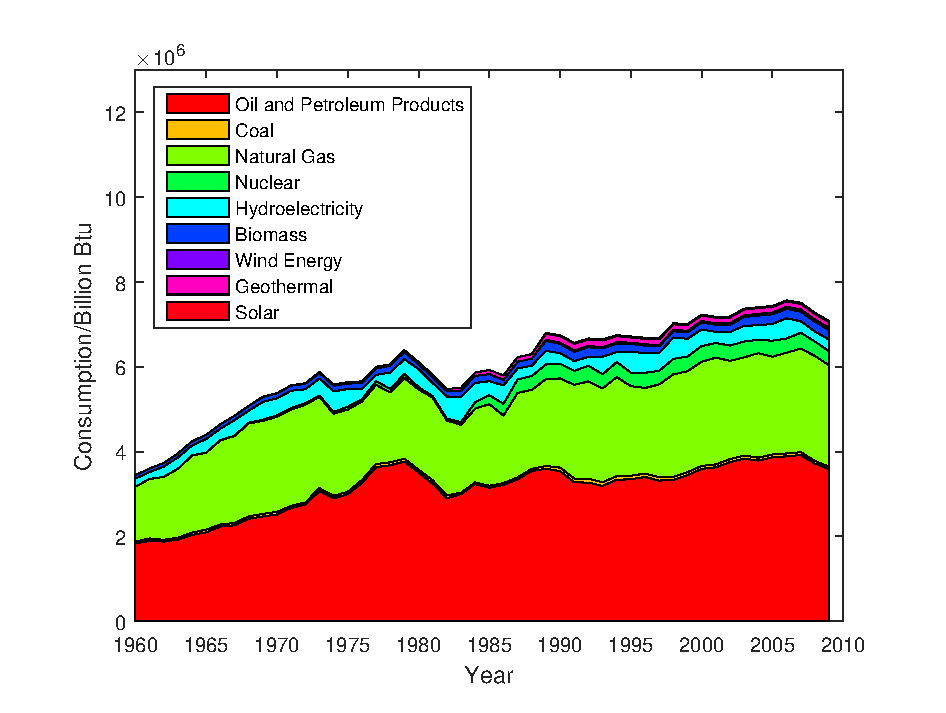
\includegraphics[scale=0.4]{figure/CAconsumption}      %以pic.jpg的0.5倍大小输出
		\end{minipage}}
		\subfigure[Energy Structure of NM]{                    %第一张子图
		\begin{minipage}{7cm}
			\centering                         %子图居中
			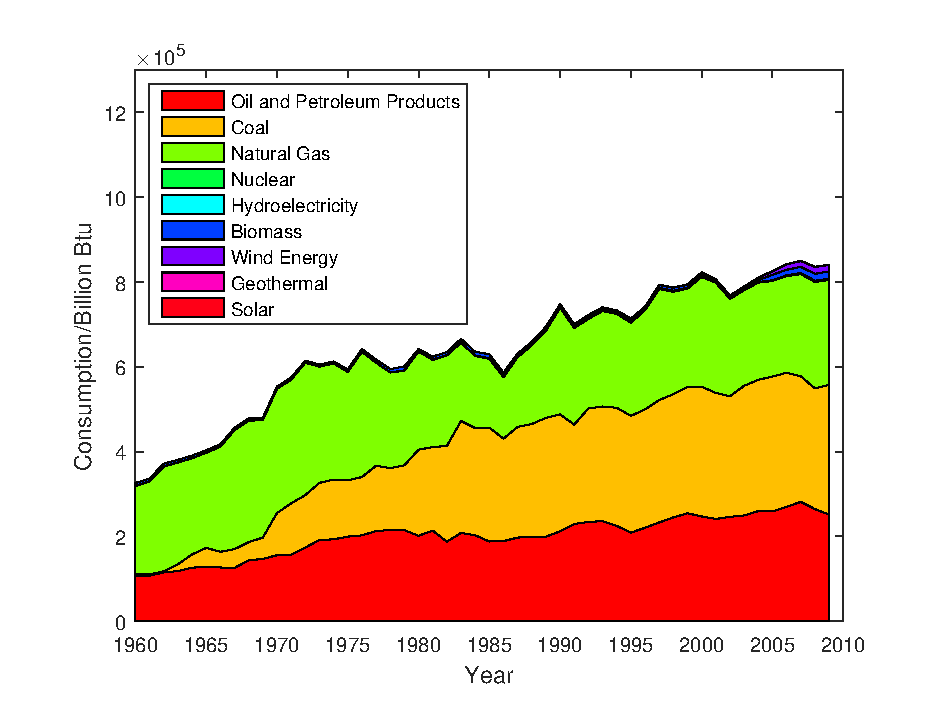
\includegraphics[scale=0.4]{figure/NMconsumption}    %以pic.jpg的0.5倍大小输出
	\end{minipage}}
	\subfigure[Energy Structure of TX]{                    %第二张子图
		\begin{minipage}{7cm}
			\centering                                     %子图居中
			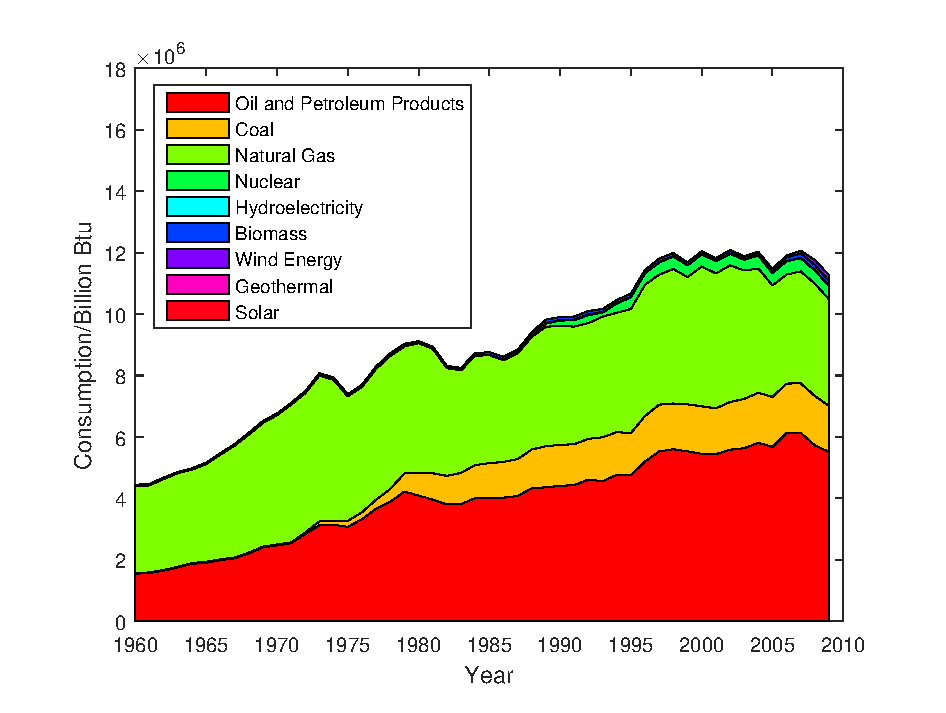
\includegraphics[scale=0.4]{figure/TXconsumption}      %以pic.jpg的0.5倍大小输出
	\end{minipage}}
	\caption{ Four-State energy profile 
	}                      %大图名称
	\label{fig:mianjitu}                                       %图片引用标记
\end{figure}
The four states has been ranked from low to high according to the total energy consumption.
\begin{itemize}
	\item In New Mexico, oil and petroleum products, coal and natural gas are the main component.New Mexico's total energy consumption is the least in the four states.
	\item In Arizona, fossil fuels have always dominated, still accounting for well over half in 2009.Although there are fluctuations, hydroelectricity and biomass have been to maintain a certain amount of consumption.
	\item In California, oil and petroleum products and natural gas also are the main component. California's energy is diverse, whose energy consumption structure include hydroelectricity, biomass, wind energy, and geothermal.
	\item In Texas, oil and petroleum products and natural gas have always dominated.The proportion of biomass and wind energy is very low.
\end{itemize}
\subsection{Analysis Model}
\subsubsection{Energy Proportion Model}
Because electricity is often consumed in time, the electricity stored in the batteries will be consumed by the business. And fossil fuels energy, various types of renewable energy (except biomass, mainly fuel ethanol) and nuclear energy will be converted into electricity,
we choose fossil fuels energy, renewable energy and nuclear energy to address data. \\
Through the analysis and integration of the data, we get the proportion of fossil fuels energy, renewable energy and nuclear energy in each state over time as shown in \autoref{fig:fenbutu}.\\
\begin{figure}[htbp]
	\centering 	                                        %居中
	\subfigure[The proportion of fossil fuels energy]{                    %第一张子图
		\begin{minipage}{7cm}
			\centering                      %子图居中
			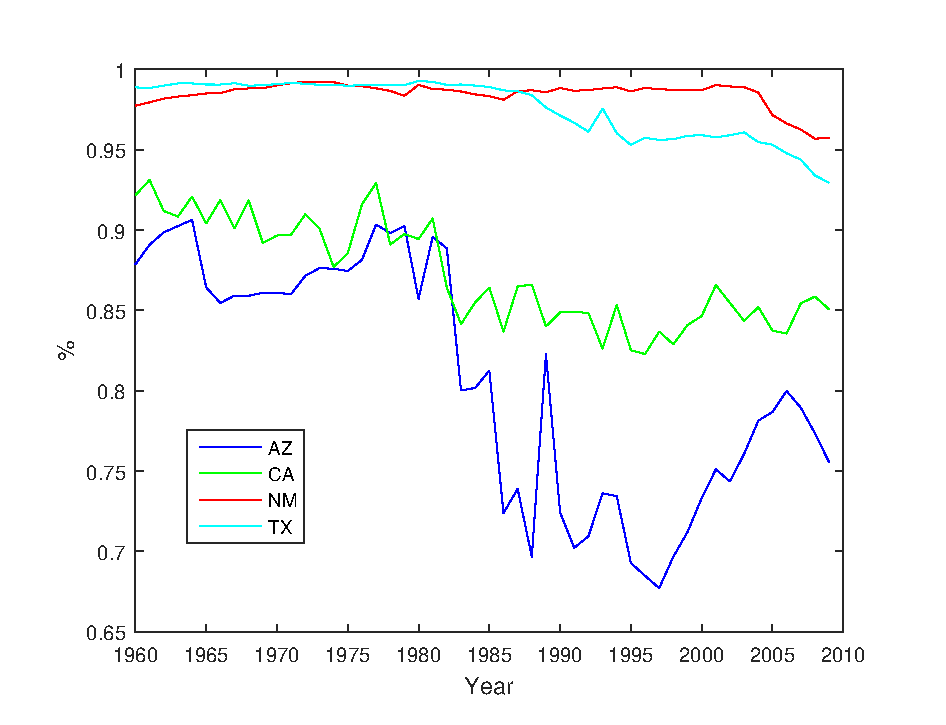
\includegraphics[scale=0.4]{figure/Thedistributionoffossilenergyovertime}    %以pic.jpg的0.5倍大小输出
	\end{minipage}}
	\subfigure[The  proportion of renewable energy]{                    %第三张子图
		\begin{minipage}{7cm}
			\centering                         %子图居中
			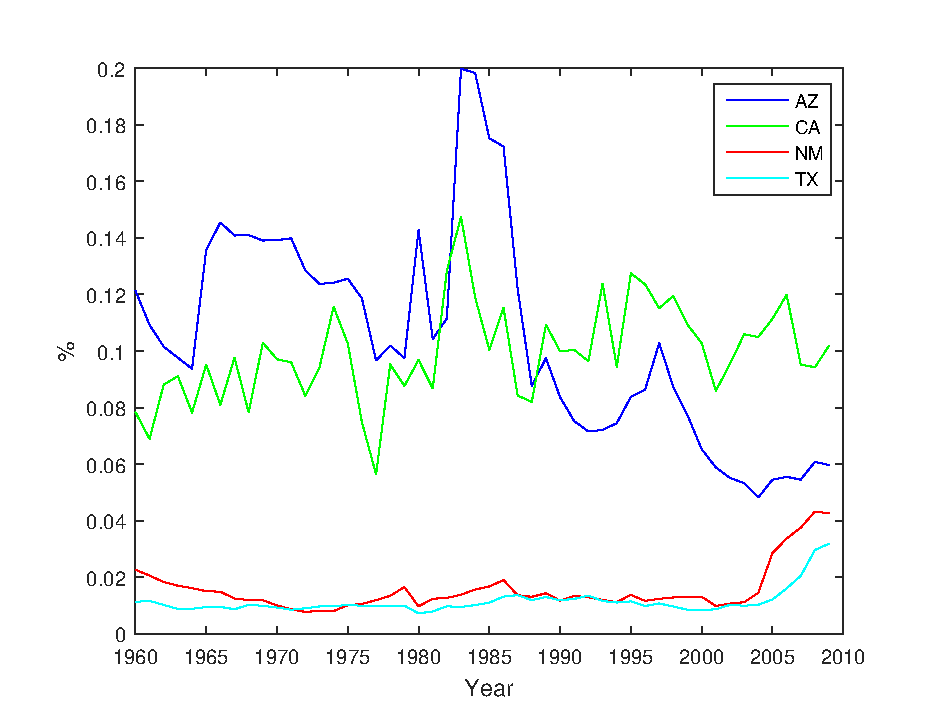
\includegraphics[scale=0.4]{figure/Thedistributionofrenewableenergyovertime}    %以pic.jpg的0.5倍大小输出
	\end{minipage}}
	\subfigure[The  proportion of nuclear energy]{                    %第二张子图
		\begin{minipage}{7cm}
			\centering                                     %子图居中
			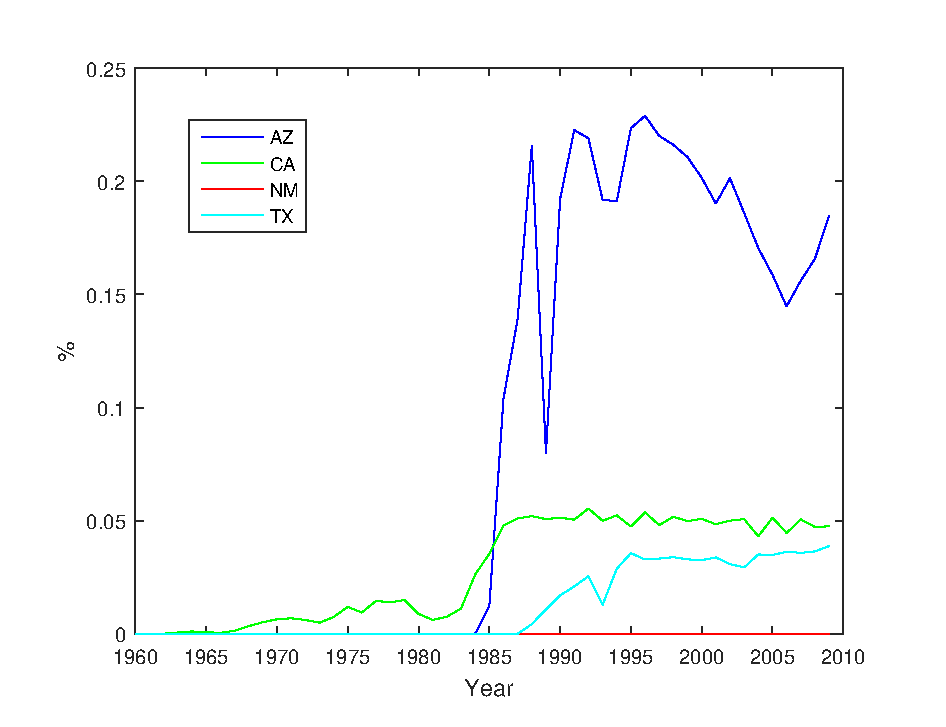
\includegraphics[scale=0.4]{figure/Thedistributionofnuclearenergyovertime}      %以pic.jpg的0.5倍大小输出
	\end{minipage}}
	\caption{The  proportion of energy in each state over time}                      %大图名称
	\label{fig:fenbutu}                                       %图片引用标记
\end{figure}
Let the proportion of energy be $ P(t) $.
We set the proportion of fossil fuels energy, renewable energy and nuclear energy as $  P_{FF}(t) $, $ P_{RE}(t) $ and $  P_{NE}(t) $.\\
Based on \autoref{eq:shiyoudaiti}, we give the conditions as follows:
\begin{numcases}{}
P_{FF}(t)+P_{RE}(t)+P_{NE}(t)=1,\notag \\
P_{FF}(t)\geqslant 0,\notag\\
P_{RE}(t)\geqslant 0,\notag\\
P_{NE}(t)\geqslant 0.
\end{numcases}
Thus, we can figure out $P(t)$. 
By using sinusoidal model to fit, we get the function expressions between prportion and time.
R-square List = [0.855, 0.8152, 0.8767, 0.9611, 0.8417, 0.2596, 0.8203, 0.6865, 0.7012, 0.9439, 0.8733] (code seen in Appendix 2)Most of R-squares are more than 0.8152, so the fuction $P(t)$ determined by sinusoidal model is very reasonable.\\
According to the proportion model, the proportion of fossil fuels in CA,NM and TX is stable over time, while AZ’s has a large fluctuation and instability.\\
When considering renewable energy, the volatility of renewable energy in AZ is large while CA’s is stable. In nearly six years, the proportion of renewable energy in NM and TX is gradually increasing, which show steady increasement of the renewable energy development momentum.\\
Nuclear energy accounted for basic stability over time, and has showed a trend of growth. The followings are the fitting formulas for the three types of energy proportion under the influence of policy, economic cycle and other factors.\\
\begin{itemize}
	\item Fossil Fuels Energy\\
	\begin{align}
	AZ:P_{FF}(t)&=5.017\sin(0.0009969t+126.7)+0.05704\sin(0.2216t-185.5)\\%R-square: 0.855
	CA:P_{FF}(t)&=0.9382\sin(0.003223+121.2)+0.02213\sin(0.1233t+10.23)\\%R-square: 0.8152
	NM:P_{FF}(t)&=1.177\sin(0.02632t+75.04)+0.1912\sin(0.06945t+118.3)\\%R-square: 0.8767
	TX:P_{FF}(t)&=0.9915\sin(0.009547t+108.4)-0.005761\sin(0.2997t-344.7)%R-square: 0.9611
	\end{align}
	\item Renewable Energy\\
	\begin{multline}
	AZ:P_{RE}(t)=0.1324\sin(0.04229t+43.67)+0.0211\sin(0.3172t-376.8)\\+0.02394\sin(0.4863t+54.64)%R-square: 0.8417
	\end{multline}
	\begin{multline}
	CA:P_{RE}(t)=0.1392\sin(0.05312t+21.74)+0.03919\sin(0.115t+27.81)\\+0.006153\sin(0.2602t6.156)%R-square: 0.2596
	\end{multline}
	\begin{multline}
	NM:P_{RE}(t)=0.03235\sin(0.07386t-19.74)+0.03528\sin(0.1421t-26.3)\\+0.0202\sin(0.198t+117.2)%R-square: 0.8203
	\end{multline}
	\begin{multline}
	TX:P_{RE}(t)=0.02556\sin(0.04159t+43.83)+0.01253\sin(0.08998t+76.51)\\+0.003882\sin(0.2536t+6.431)%R-square: 0.6865
	\end{multline}
	\item Nuclear Energy\\
	\begin{align}
	AZ:P_{NE}(t)&=0.728\sin(0.02875t+200.4)+0.2046\sin(0.1376t+249.5)\\%R-square: 0.7012
	CA:P_{NE}(t)&=0.0606\sin(0.03157t+63.55)+0.01022\sin(0.2172t-173.5)\\%R-square: 0.9439
	TX:P_{NE}(t)&=0.0377\sin(0.07327t+149.9)+0.004349\sin(0.3589t-123.7)%R-square: 0.8733
	\end{align}
\end{itemize}
Note:Because there is no nuclear power plant in NM, we think its nuclear energy proportion is always zero.
\subsubsection{Growth Rate Model}
For a given state, we describe the state's energy development by defining variables for growth rates.\\
Now define the concept of growth rate, set the growth rate $ v $ as a function of year(time).\\
\begin{align}
v(t)=\dfrac{c(t)-c(t-1)}{c(t-1)}
\end{align}
We use Moving Average in Time Series to get 1963-2007 energy consumption called $ c(t) $\cite{mova}, whose goal is to eliminate stochastic disturbances and year-to-year interactions. And we take the real consumption called $ \mathit{rc} $ from the excel table.\\
\begin{align}
c(t)=\dfrac{\sum_{i=t-2}^{t+2}\mathit{rc(t)}}{N}(N=5),\qquad i\geq 3
\end{align}


Thus, we can figure out $ v(t) $. By using sinusoidal model to fit, we get the function expressions between growth rate and time. Most of R-squares are more than 0.653, so the fuction $  v(t) $ determined by sinusoidal model vis very reasonable.(code seen in appendices 3)
\begin{itemize}
	\item The Growth Rate of Renewable Energy\\
	\setlength\multlinegap{0em}
	\setlength\multlinetaggap{6em}
	\begin{multline}
	AZ:v(t)=0.1324\sin(0.04229t+43.67)+0.0211\sin(0.3172t-376.8)\\+0.02394\sin(0.4863t+54.64)%R-square: 0.8417
	\end{multline}
	\begin{multline}
	CA:v(t)=0.1392\sin(0.05312t+21.74)+0.03919\sin(0.115t+27.81)\\+0.006153\sin(0.2602t6.156)%R-square: 0.2596
	\end{multline}
	\begin{multline}
	NM:v(t)=0.03235\sin(0.07386t-19.74)+0.03528\sin(0.1421t-26.3)\\+0.0202\sin(0.198t+117.2)%R-square: 0.8203
	\end{multline}
	\begin{multline}
	TX:v(t)=0.02556\sin(0.04159t+43.83)+0.01253\sin(0.08998t+76.51)\\+0.003882\sin(0.2536t+6.431)%R-square: 0.6865
	\end{multline}
	\begin{figure}[htbp]
		\centering                                             %居中
		\subfigure[Growth rate of energy consumption of AZ]{                    %第一张子图
			\begin{minipage}{7cm}
				\centering                         %子图居中
				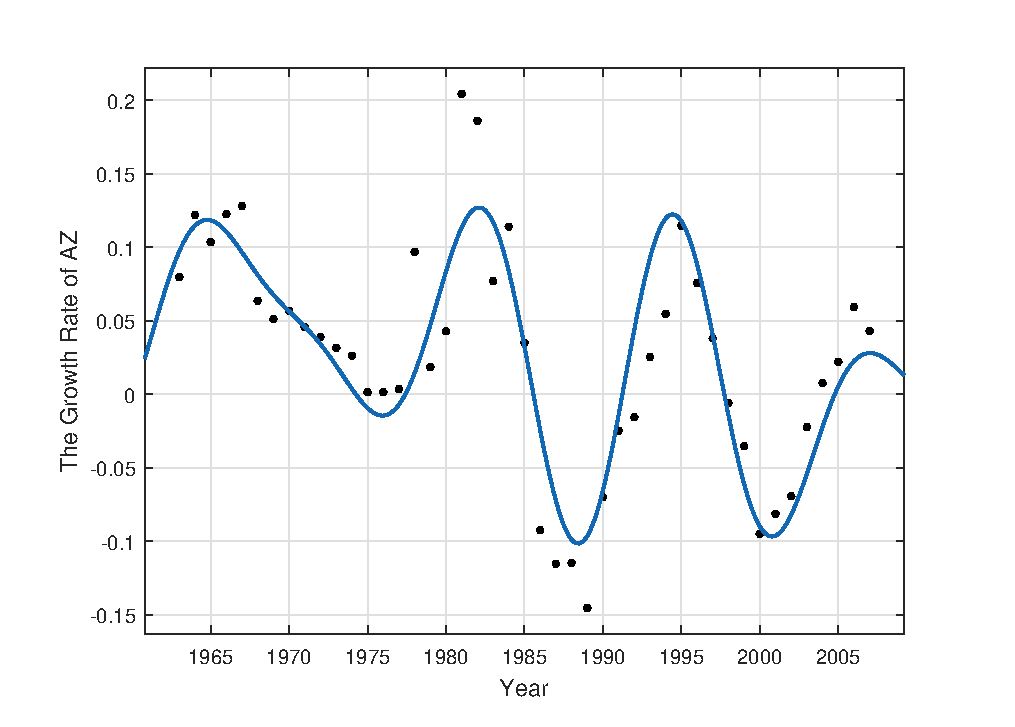
\includegraphics[scale=0.4]{figure/AZGrowthRate}    %以pic.jpg的0.5倍大小输出
		\end{minipage}}
		\subfigure[Growth rate of energy consumption of CA ]{                    %第二张子图
			\begin{minipage}{7cm}
				\centering                                     %子图居中
				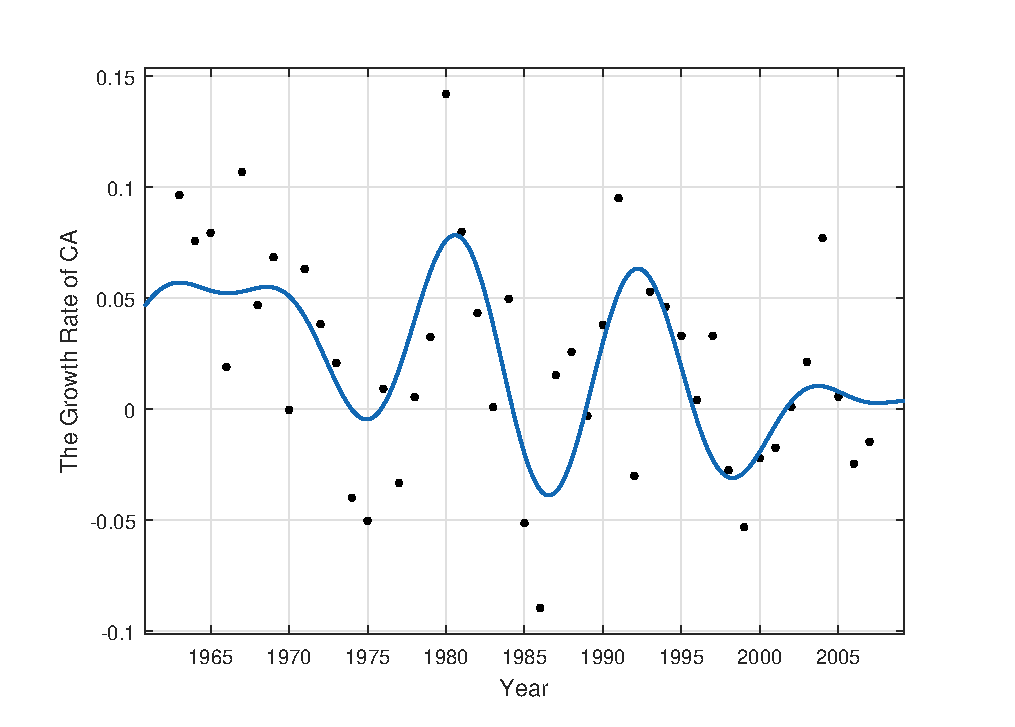
\includegraphics[scale=0.4]{figure/CAGrowthRate}      %以pic.jpg的0.5倍大小输出
		\end{minipage}}
		\subfigure[Growth rate of energy consumption of NM]{                    %第三张子图
			\begin{minipage}{7cm}
				\centering                         %子图居中
				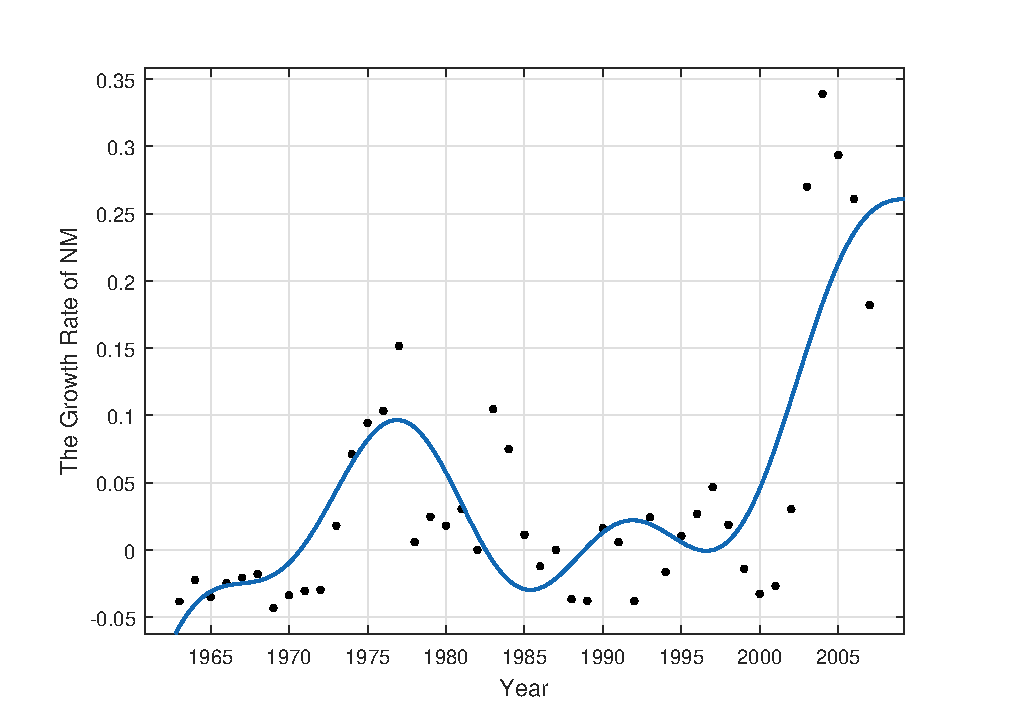
\includegraphics[scale=0.4]{figure/NMGrowthRate}    %以pic.jpg的0.5倍大小输出
		\end{minipage}}
		\subfigure[Growth rate of energy consumption of TX]{                    %第四张子图
			\begin{minipage}{7cm}
				\centering                                     %子图居中
				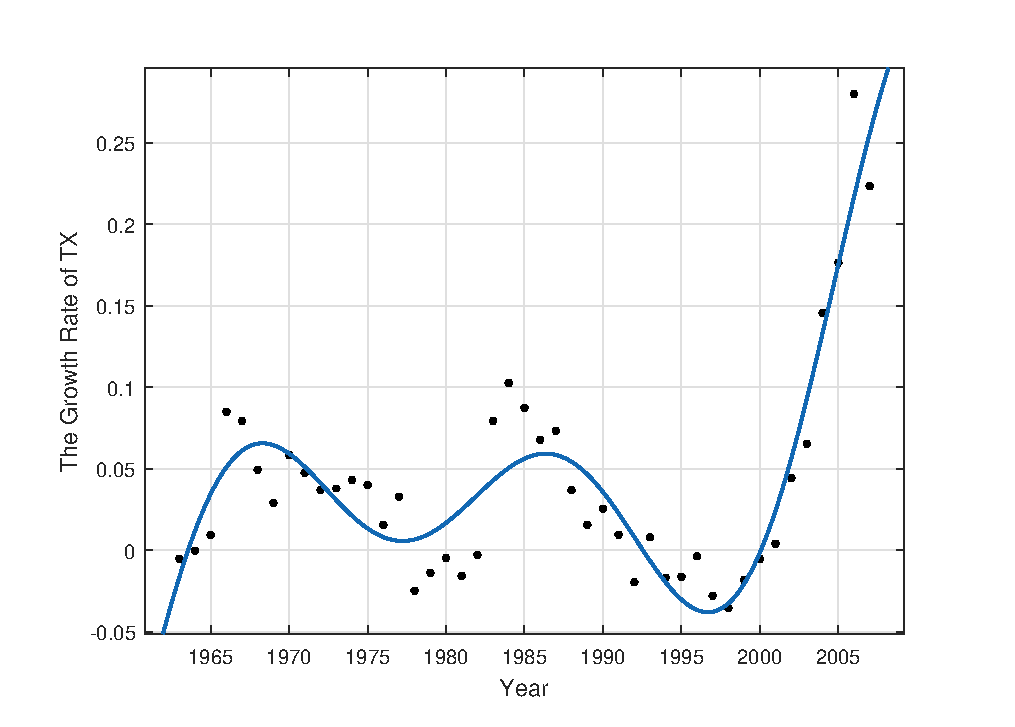
\includegraphics[scale=0.4]{figure/TXGrowthRate}      %以pic.jpg的0.5倍大小输出
		\end{minipage}}
		\caption{Four-State growth rate of energy consumption	}                      %大图名称
		\label{fig:GrowthRateRenewable}                                       %图片引用标记
	\end{figure}
   \item The Growth Rate of Fossil Fuel Energy\\
   \begin{multline}
   AZ:v(t)=0.03936\sin(0.04589t+49.21)+0.0287\sin(0.2133t-142.3)\\+0.009263\sin(0.431t-289.9)%R-square: 0.791
   \end{multline}
   \begin{multline}
   CA:v(t)=0.03393\sin(0.0602t+21.27)+0.02562\sin(0.1332t+17.44)\\+0.01385\sin(0.5719t-4.184)%R-square: 0.7333
   \end{multline}
   \begin{multline}
   NM:v(t)=0.05732\sin(0.02103t+99.33)+0.0175\sin(0.189t-93.12)\\+0.01297\sin(0.6878t+53.84)%R-square: 0.7552
   \end{multline}
   \begin{multline}
   TX:v(t)=0.03289\sin(0.0466t+48.2)+0.01849\sin(0.2133t-141.5)\\+0.01206\sin(0.6927t+45.17)%R-square:  0.8856
   \end{multline}
   \item The Growth Rate of Nuclear Energy\\
   \begin{multline}
   AZ:v(t)=0.03289\sin(0.0466t+48.2)+0.01849\sin(0.2133t-141.5)\\+0.01206\sin(0.6927t+45.17)%R-square:  0.9064
   \end{multline}
   \begin{multline}
   CA:v(t)=2.219\sin(0.1487t-154.8)+0.2715\sin(0.2861t-0.7948)\\+2.218\sin(0.1615t-38.96)%R-square: 0.673
   \end{multline}
   \begin{multline}
   TX:v(t)=0.1818\sin(0.2526t-113.4)+0.1604\sin(0.3707t+42.78)\\+0.0297\sin(1.902t+120.8)%R-square:  0.9309
   \end{multline}
\end{itemize}
It can be seen from the figure above that the consumption of renewable energy has a cyclical change over time, but it has shown a significant upward in the past 10 years in NM and TX. 
\subsubsection{Influential Factors of the similarities and differences}
According to our energy profile model and the data provided, we select industry and population as influential factors to analyze the similarities and differences about usage of cleaner, renewable energy sources between the four states. 
\begin{itemize}
	\item Sector\\
	The similarities and differences between the four states can be seen from the degree of demand for energy consumption in various industries.\\ To determine the industrial factors over time, we chose the industry,commerce and residential industries. For the transportation industry, after analyzing the data, the impact on renewable energy is negligible. The largest proportion in CA is 1.34\%, considering the contribution rate, we ignore it.\\
	We give the definition of the impact factor. Since the energy consumption of each year is known, and we assume that the impact factor is a function of time $ Q_{1}(t) $, $ Q_{2}(t) $, $ Q_{3}(t) $ are defined as the impact factor.
	\begin{gather}
	c_{1} \cdot Q_{1}(t)+c_{2} \cdot Q_{2}(t)+c_{3} \cdot Q_{3}(t)=\mathit{rc(t)}
	\end{gather}
The similarity is that the ratio of impact factors of AZ, NM, TX called as $ Q_{1}(t) $, $ Q_{2}(t) $, $ Q_{3}(t) $ is $ 3.412:1:1 $.\\
The difference is that the ratio of impact factors of CA states changes over time, with the attached illustrations of CA shown in \autoref{fig:Industry}.(code seen in Appendices 6)
	\begin{figure}[h]
		\centering
		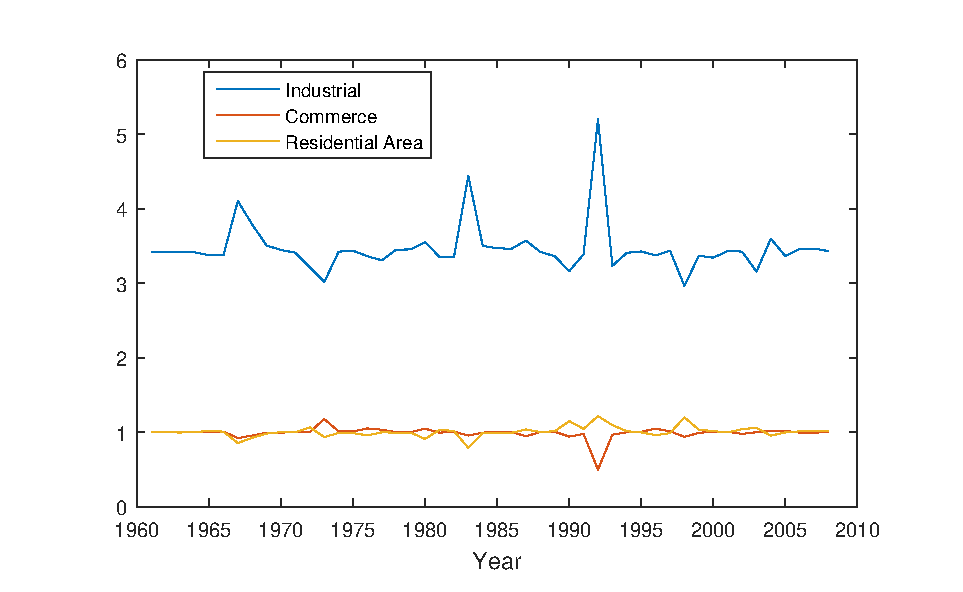
\includegraphics[width=12cm]{figure/Factorsofthesimilaritiesanddifferences}
     	\caption{The impact factors of CA changes over time}
		\label{fig:Industry}
	\end{figure}
	\item Population\\
		We assume that the value of dollar is stable remain unchanged for several years(2000-2005).\\
	We use the IPAT formula and the revised "Laspeyres" exponential decomposition method to analyze the impact of population growth on total energy consumprtion gowth.\cite{IPAT}\\
	We take $ \Delta $ as the change from the end of the year to the beginning.\\
	In the model, $ \Delta TPOPP$ can represent the impact of population size on energy consumption.\\
	The population of these four states increases approximately linearly over time, and the rate of increase is positively correlated with their population base.
	\begin{align}
	\Delta TETCB&=TETCB_{t}-TETCB_{0}\notag\\&=\Delta TPOPP^{effects}+\Delta A^{effects}+\Delta TETGR^{effects}
	\end{align}
	\setlength\multlinegap{4em}
	\setlength\multlinetaggap{8em}
	\begin{multline}
	\Delta TPOPP^{effects}=\Delta TPOPP\cdot A_{0}\cdot TETGR_{0}\\
	+\frac{1}{2}\left ( \Delta TPOPP\cdot \Delta A\cdot TETGR_{0} \right ) \\
	+\frac{1}{2}\left ( \Delta TPOPP\cdot A_{0}\cdot \Delta TETGR \right )\\
	+ \frac{1}{3}\left ( \Delta TPOPP\cdot \Delta A\cdot \Delta TETGR \right)
	\end{multline}
	\begin{multline}
	\Delta A^{effects}= TPOPP_{0}\cdot \Delta A\cdot TETGR_{0}\\
	+\frac{1}{2}\left ( \Delta TPOPP\cdot \Delta A\cdot TETGR_{0} \right ) \\
	+\frac{1}{2}\left ( TPOPP_{0}\cdot \Delta A\cdot \Delta TETGR \right )\\
	+\frac{1}{3}\left ( \Delta TPOPP\cdot \Delta A\cdot \Delta TETGR \right )
	\end{multline}
	\begin{multline}
	\Delta TETGR^{effects}= TPOPP_{0}\cdot A_{0}\cdot \Delta TETGR\\
	+\frac{1}{2}\left ( TPOPP_{0}\cdot \Delta A\cdot \Delta TETGR \right )\\
	+\frac{1}{2}\left ( \Delta TPOPP\cdot A_{0}\cdot \Delta TETGR \right ) \\
	+\frac{1}{3}\left ( \Delta TPOPP\cdot \Delta A\cdot \Delta TETGR \right )
	\end{multline}	
	However, the disaggregation analysis structure based on the population scale model shows that the energy consumption growth in each state has great volatility in growth of population size.\\
	Positive effect shows that Americans have a lot of differences in energy usage. The peak $ \Delta TETCB $ far above 100\% between 1978 and 2009 can also reflect the wealth distribution of Americans. The energy consumption characteristics of high-income groups play a significant role in the overall energy consumption structure.\\
	After excluding the largest peak, we find that the increase in population size in AZ and CA has a negative effect on the increase in energy consumption while the increase in population size in NM and TX has a positive effect on the increase in energy consumption.
	\begin{figure}[h]
		\centering                                             %居中
		\subfigure[Energy consumption changes with population of AZ]{                    %第一张子图
			\begin{minipage}{7cm}
				\centering                         %子图居中
				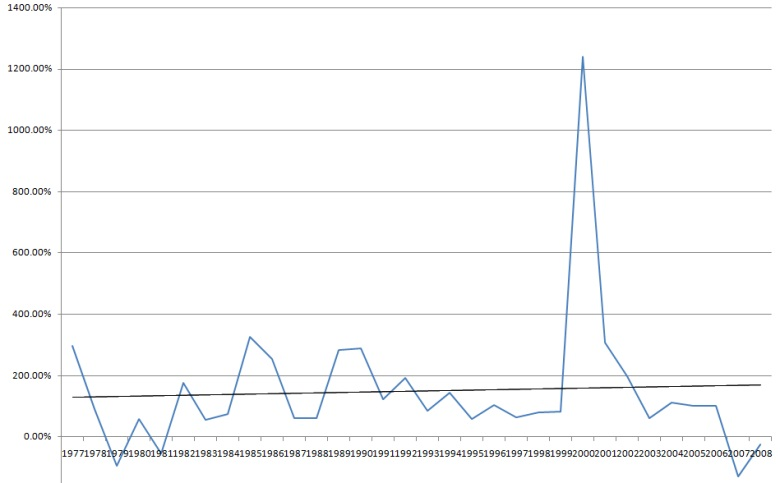
\includegraphics[scale=0.38]{figure/AZrenkouguimo2}    %以pic.jpg的0.5倍大小输出
		\end{minipage}}
		\subfigure[Energy changes with population of CA ]{                    %第二张子图
			\begin{minipage}{7cm}
				\centering                                     %子图居中
				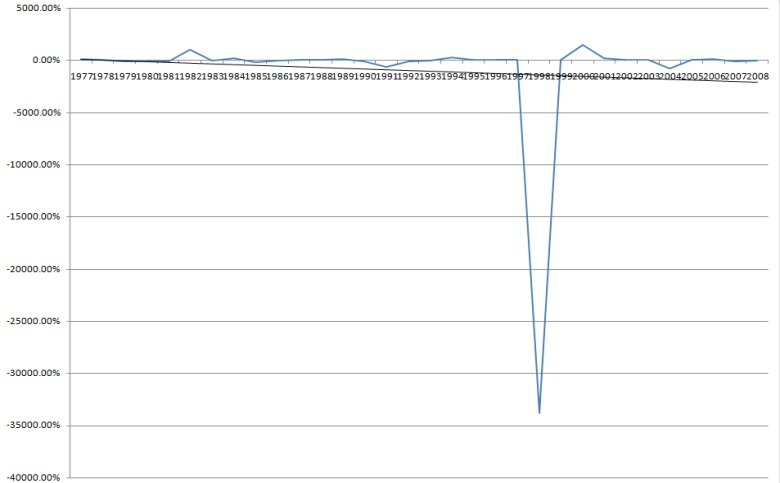
\includegraphics[scale=0.38]{figure/CArenkouguimo2}      %以pic.jpg的0.5倍大小输出
		\end{minipage}}
		\subfigure[Energy changes with population of NM]{                    %第三张子图
			\begin{minipage}{7cm}
				\centering                         %子图居中
				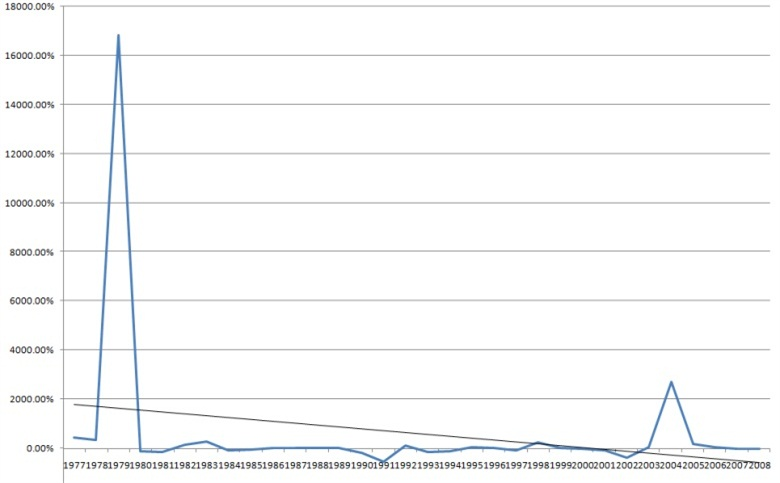
\includegraphics[scale=0.38]{figure/NMrenkouguimo2}    %以pic.jpg的0.5倍大小输出
		\end{minipage}}
		\subfigure[Energy changes with population of TX]{                    %第四张子图
			\begin{minipage}{7cm}
				\centering                                     %子图居中
				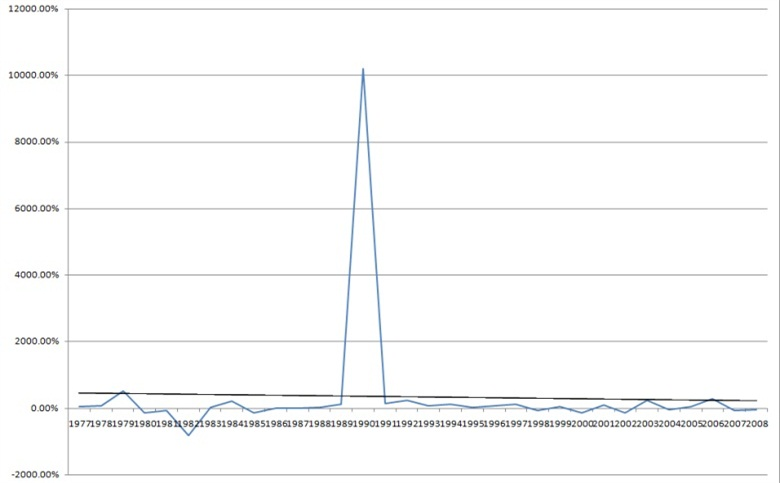
\includegraphics[scale=0.38]{figure/TXrenkouguimo2}      %以pic.jpg的0.5倍大小输出
		\end{minipage}}
		\caption{Energy changes with population of four states}                      %大图名称
		\label{fig:Population}                                       %图片引用标记
	\end{figure}
\end{itemize}
\subsubsection{Evaluation Criteria for the best Profile}
We select the appropriate indicators, establish an credible evaluation criteria to determine which of the four states appeared to have the “best” profile for use of cleaner, renewable energy in 2009.\\
Through the analysis of the data, we have integrated distribution in cleaner and renewable energy. Various types of renewable energy (except biomass, mainly fuel ethanol) and nuclear energy will be converted into electricity.
From the perspective of distribution, the share of electricity in the four states is the largest and more representative, so we choose the energy source of electricity as the basis for analysis.\\ Then we select the average price, import expenditure size, size of productivity as the evaluation criteria (they are highly correlated with energy efficiency) according to literature we view.\cite{evaluation}
In order to get the weight vector, we need to compute the weight of the
three factors.
Thus, we can figure out that the weight vector  $ B=\begin{bmatrix}
0.259&0.0653&0.6757
\end{bmatrix}  $.
Finally, in consistency check, the consistency index CI =  0.0098 < 0.10, which
means that the weight determined by AHP is very reasonable.\cite{AHP}(code seen in Appendix 7)
Therefore, we established the three criteria of paired comparison judgment matrix.\\
\begin{center}
	The average price of electricity paired comparison judgment matrix
\end{center}
\[W_{1}= \begin{bmatrix}
1	& 	0.719854804		& 1.168808758	& 	0.958872523\\
1.389169031		& 1		& 1.62367293	& 	1.332036014\\
0.85557196	& 	0.615887585	& 	1	& 	0.820384444\\
1.042891496	& 	0.750730453	& 	1.218940714		& 1
\end{bmatrix} 
\]
\begin{center}
	The import expenditure size of electricity  paired comparison judgment matrix
\end{center}
\[ W_{2}=\begin{bmatrix}
1&	0.040360221	&4.525931207&	0.27494136\\
24.77687143	&1&	112.1384156&	6.812186739\\
0.220949006&	0.008917551&	1&	0.06074802\\
3.637139201&	0.146795741&	16.46144181&	1
\end{bmatrix} \] 
\begin{center}
	The size of productivity paired comparison judgment matrix
\end{center}
\[W_{3}= \begin{bmatrix}
	1 & 0.282887 & 3.39227 & 0.212667 \\ 
	3.534976 & 1 & 11.99159 & 0.751772 \\ 
	0.294788 & 0.083392 & 1 & 0.062692 \\ 
	4.70219 & 1.33019 & 15.9511 & 1
\end{bmatrix}  \]
\begin{center}
	The four-state weights matrix
\end{center}
\[ A= \begin{bmatrix}
0.2332 & 0.0337 & 0.1049\\ 
0.324 & 0.8361 & 0.3709 \\ 
0.1995 & 0.0075 & 0.03.9 \\ 
0.2432& 0.1227& 0.4933
\end{bmatrix}\]
\begin{gather}
C=A*B^{T}
\end{gather}

The largest total sort weight is in \textbf{TX} whose total sort weight is 0.4043. Therefore, TX has the “best” profile in 2009.
\begin{table}[h]
	\centering
	\caption{The Total Hierarchy}
	\label{my-label}
	\begin{tabular}{|c|l|r|r|r|r|}
		\hline
		\multicolumn{2}{|c|}{Standard}               & \multicolumn{1}{l|}{Average price} & \multicolumn{1}{l|}{Import expenditures} & \multicolumn{1}{l|}{Productivity} & \multicolumn{1}{l|}{\multirow{2}{*}{Total sort weight}} \\ \cline{1-5}
		\multicolumn{2}{|c|}{Standard layer weights} & 0.259                              & 0.0653                                   & 0.6757                            & \multicolumn{1}{l|}{}                                   \\ \hline
		\multirow{4}{*}{four-state weights}   & AZ   & 0.2332                             & 0.0337                                   & 0.1049                            & 0.1335                                                  \\ \cline{2-6} 
		& CA   & 0.324                              & 0.8361                                   & 0.3709                            & 0.3891                                                  \\ \cline{2-6} 
		& NM   & 0.1995                             & 0.0075                                   & 0.0309                            & 0.073                                                   \\ \cline{2-6} 
		& TX   & 0.2432                             & 0.1227                                   & 0.4933                            & 0.4043                                                  \\ \hline
	\end{tabular}
\end{table}
\subsubsection{Predict the energy profile of each state for 2025 and 2050}	
\begin{equation}
v^{-}(t) \leq v(t) \leq v^{+}(t)
\end{equation}
We address that $ v(t) $ cannot be in the range of 80\% to 100\% of the boundary value for many years based on the absence of policy.\\
Predictive Result by Energy Proportion Model and Growth Rate Model to predict the energy profile of each state, for 2025 and 2050 in the absence of any policy changes by each governor’s office.\\
After comparing the predictions of the two models, we find that the results based on Growth Rate Model are basically smaller than that based on Energy Proportion Model, and the difference will be greater when the prediction is further away. \\
This is because Growth Rate Model considers the cyclicality and volatility of the growth rate, and the cyclicality and volatility can lead to negative value of growth rate in some years while the total consumption used in Energy Proportion Model is approximately linear linearly proportional to time.
This inevitably leads to differences, and the longer the forecast year, the greater the difference. \\
We also find that the proportion of renewable energy in AZ was up to 33\%, and we believe that the proportion is obviously large, which may not be consistent with the actual situation.
Various numerical value for unity (Billion Btu)

% Please add the following required packages to your document preamble:
% \usepackage{multirow}
\begin{table}[htbp]
	\centering
	\caption{The energy consumption  predicted by Energy Proportion Model}
	\label{my-label}
	\begin{tabular}{|c|l|r|r|r|r|}
		\hline
		Consumption         & \multicolumn{1}{c|}{Year} & \multicolumn{1}{c|}{Total} & \multicolumn{1}{c|}{Fossil} & \multicolumn{1}{c|}{Renewable} & \multicolumn{1}{c|}{Nuclear} \\ \hline
		\multirow{2}{*}{AZ} & 2025                      & 2320000                    & 1621957.268                 & 219190.8396                    & 478851.8922                  \\ \cline{2-6} 
		& 2050                      & 3130000                    & 1730704.623                 & 1038752.306                    & 360543.0705                  \\ \hline
		\multirow{2}{*}{CA} & 2025                      & 8827500                    & 7444779.641                 & 893501.5493                    & 489218.81                    \\ \cline{2-6} 
		& 2050                      & 10555000                   & 8140122.189                 & 1663263.361                    & 751614.4503                  \\ \hline
		\multirow{2}{*}{NM} & 2025                      & 1034925                    & 947674.8402                 & 87250.15979                    & 0                            \\ \cline{2-6} 
		& 2050                      & 1275850                    & 1138215.545                 & 137634.4553                    & 0                            \\ \hline
		\multirow{2}{*}{TX} & 2025                      & 15502500                   & 13591078.48                 & 962591.0042                    & 948830.5125                  \\ \cline{2-6} 
		& 2050                      & 19505000                   & 14375512.95                 & 1915932.14                     & 3213554.907                  \\ \hline
	\end{tabular}
	\label{tab:ProPredict}%
\end{table}
\begin{table}[htbp]
	\centering
	\caption{The energy consumption predicted by Growth Rate Model}
	\label{my-label}
	\begin{tabular}{|c|l|r|r|r|r|}
		\hline
		Consumption         & \multicolumn{1}{c|}{Year} & \multicolumn{1}{c|}{Total} & \multicolumn{1}{c|}{Fossil} & \multicolumn{1}{c|}{Renewable} & \multicolumn{1}{c|}{Nuclear} \\ \hline
		\multirow{2}{*}{AZ} & 2025                      & 2248319.93                 & 1591602.402                 & 214609.231                     & 442108.2977                  \\ \cline{2-6} 
		& 2050                      & 2974605.804                & 2487110.463                 & 289309.8205                    & 198185.5211                  \\ \hline
		\multirow{2}{*}{CA} & 2025                      & 8221835.779                & 6843119.367                 & 958467.7855                    & 420248.6265                  \\ \cline{2-6} 
		& 2050                      & 9307875.255                & 7532637.203                 & 1607317.613                    & 167920.4387                  \\ \hline
		\multirow{2}{*}{NM} & 2025                      & 920543.7673                & 834833.1874                 & 85710.5799                     & 0                            \\ \cline{2-6} 
		& 2050                      & 924918.767                 & 831442.2678                 & 93476.49919                    & 0                            \\ \hline
		\multirow{2}{*}{TX} & 2025                      & 13271821.75                & 11558362.78                 & 883172.252                     & 830286.712                   \\ \cline{2-6} 
		& 2050                      & 14799231.47                & 11794310.35                 & 1123835.433                    & 1881085.688                  \\ \hline
	\end{tabular}
\label{tab:GroPredict}%
\end{table}

%	\label{tab:ProPredict}%

